
% Cal Poly Thesis
% 
% based on UC Thesis format
%
% modified by Mark Barry 2/07.
%




\documentclass[12pt]{ucthesis}


\usepackage{url}

    \usepackage[pdftex]{graphicx}
    % Update title and author below...
    \usepackage[pdftex,plainpages=false,breaklinks=true,colorlinks=true,urlcolor=blue,citecolor=blue,%
                                       linkcolor=blue,bookmarks=true,bookmarksopen=true,%
                                       bookmarksopenlevel=3,pdfstartview=FitV,
                                       pdfauthor={Justin Phillips},
                                       pdftitle={Functional-Reactive-Musician},
                                       pdfkeywords={thesis, masters, cal poly}
                                       ]{hyperref}
    %Options with pdfstartview are FitV, FitB and FitH
    \pdfcompresslevel=1



\usepackage{amssymb}
\usepackage{amsmath}
\usepackage[letterpaper]{geometry}
\usepackage[overload]{textcase}



\bibliographystyle{abbrv}

\setlength{\parindent}{0.25in} \setlength{\parskip}{6pt}

\geometry{verbose,nohead,tmargin=1.25in,bmargin=1in,lmargin=1.5in,rmargin=1.3in}

\setcounter{tocdepth}{2}


% Different font in captions (single-spaced, bold) ------------
\newcommand{\captionfonts}{\small\bf\ssp}

\makeatletter  % Allow the use of @ in command names
\long\def\@makecaption#1#2{%
  \vskip\abovecaptionskip
  \sbox\@tempboxa{{\captionfonts #1: #2}}%
  \ifdim \wd\@tempboxa >\hsize
    {\captionfonts #1: #2\par}
  \else
    \hbox to\hsize{\hfil\box\@tempboxa\hfil}%
  \fi
  \vskip\belowcaptionskip}
\makeatother   % Cancel the effect of \makeatletter
% ---------------------------------------




\begin{document}

% Declarations for Front Matter

% Update fields below!
\title{A Functional Reactive Improviser}
\author{Justin Phillips}
\degreemonth{December} \degreeyear{2010} \degree{Master of Science}
\defensemonth{December} \defenseyear{2010}
\numberofmembers{3} \chair{John Clements, Ph.D.} \othermemberA{Aaron Keen, Ph.D.} \othermemberB{Zo\"{e} Wood, Ph.D.} \field{Computer Science} \campus{San Luis Obispo}
\copyrightyears{seven}



\maketitle

\begin{frontmatter}

% Custom made for Cal Poly (by Mark Barry, modified by Andrew Tsui).
\copyrightpage

% Custom made for Cal Poly (by Andrew Tsui).
\committeemembershippage

\begin{abstract}

%This is where the abstract goes.  Hopefully this document will serve as an example for preparing a Cal Poly Master's thesis.  It was thrown together pretty quickly.  A lot more neat LaTeX features, help, and examples can be found on the web.  Here is one: http://en.wikibooks.org/wiki/LaTeX

%For developing LaTeX documents in the Windows environment, I use TeXnicCenter (http://www.toolscenter.org/).  A simple WYSIWYG LaTeX editor (though I had problems getting it to work with this thesis format) is \textbf{LyX} (http://www.lyx.org/).

%I use \textbf{InkScape} (http://www.inkscape.org/) to create any drawings/figures needed.  It is a free vector graphics editor that is very powerful and popular.  There is an example figure produced with InkScape in Figure~\ref{fig:inkscape-example}.  InkScape can export images in many different formats.  Export your images as PDF or EPS and put into your LaTeX document.  If you're creating a PDF document with \textbf{pdflatex}, then export as a PDF image.  If you're creating PostScript then export as EPS.  Rasterized images such as JPEG can also be easily included in LaTeX.

%LaTeX can also produce nice equations.  Did you know that $\sum_{n=0}^{\infty} \frac{(-1)^n}{2n+1} = \frac{1}{1} - \frac{1}{3} + \frac{1}{5} - \frac{1}{7} + \frac{1}{9} - \cdots = \frac{\pi}{4}$ ?  A non-inline equation can be found in Figure~\ref{eqn:example}.  I treated my equations as figures but they can be treated specially as Equations.

%An example of a table can be found in Table~\ref{table:performance}.

%The bibliography section is very easy to create.  When gathering references, I used the ACM digital library (http://portal.acm.org/portal.cfm) to grab the Bibtex entries.  Papers in the digital library have Bibtex entries ready to be copied and pasted into your bibliography.  Create a separate file called something like ``bibliography.bib'' and paste in your Bibtex entries.  LaTeX (and Bibtex) generate your bibliography section for you -- very easy! I can cite references very easily.  Here is a paper called \emph{Dual contouring of hermite data}~\cite{DualContouring}.  Here is a paper called \emph{Surface simplification using quadric error metrics}~\cite{QuadricErrorMetrics}.  I've also cited software located at some websites \cite{NormalMapper}~\cite{nVidiaMelody}.

This thesis describes an event driven, reactive musical performer. It takes a different approach to the problem of creating melodic improvisation.~\cite{bob} In solving this problem in the FrTime language, a signal handler was developed to maintain the possible values in the future and perform a computation over these values to decide which value should be the correct answer at the time that it is needed. At the end of the document an experiment is performed with three different performers in hopes of discovering the 'best' improviser. The framework created is extensible and uses a Haskore like syntax for describing music. New performers and improvisers can be created without any substantial change to the framework. This framework was written for the DrRacket environment and provides a MIDI extension for use with DrRacket on Mac OS X and Linux. 

\end{abstract}

%\begin{acknowledgements}

%   Thank you...

%\end{acknowledgements}


\tableofcontents


\listoftables

\listoffigures

\end{frontmatter}

\pagestyle{plain}




\renewcommand{\baselinestretch}{1.66}


% ------------- Main chapters here --------------------

%TODO : : Results FRP Research Implementation REDUX
%TODO : : Thurs - Intro Conclusion Abstract FutureWork Redux
%TODO : : Fri - read it over, send it off.



\chapter{Introduction}
\label{intro}

Musicians need accompaniment and sometimes it is challenging to find fellow musicians to play with. This thesis addresses this issue by providing a programmable computer performer that plays music with a human performer who is performing on a MIDI instrument connected to the computer. The implementation takes advantage of the reactive programming by creating an event driven performer that reacts to each input received from the MIDI instrument. The goal is to create a framework that handles all of the parts of performing music that are not unique to a performer and allow developers to create many performers. 

At the same time, this thesis addresses the issue of providing the highest payoff or reward at every point in time via a reactive behavior. A module is developed that controls a user created behavior which is associated with a user provided maximum value function. The behavior's value is then set to values that the user has added and have been processed by the value function. This interface is used to provide the most musically pleasing output but has further implications into other domains. 

The next chapter addresses work, both in the field of computers and music, and in the functional reactive domain. A short crash course in music theory is provided as well. Following that is a description of the implementation and problems that arose and how they were solved. The fourth section describes an experiment in programming different performers followed by a section describing the results of these experiments. Future work is discussed and followed by a conclusion.

\chapter{Related Work}
\label{rw}

The following section is organized as follows : a short introduction to western music theory, followed by a description of Haskore, related works that deal with music, and finally the work done with Functional Reactive languages.

\section{Music Theory}
\label{rw:music-theory}

Firstly, understanding music theory requires no ability to hear difference in pitch or rhythm. Specifically, this section discusses Western music theory at a very high level so that the reader can understand how the system works. 

Music can be described as a series of notes happening at discrete times. More specifically, a piece of music consists of four characteristics: time signature, tempo, key signature and form.

The time signature describes how many beats are in a measure and what kind of beat they are. For example, 3/4 and 4/4 are common time signatures. 3/4 means that there are three quarter notes in each measure. A measure is the space on the sheet of music between two vertical lines. Many measures make up a piece of music. 4/4 then would be the same, except that there would be four quarter notes in each measure. The rate at which the beats happen in time is called the tempo and is measured in beats per minute. So a song in 4/4 can have a tempo of 120 or 60 or any other number. In the case where the tempo was 60 that would mean every quarter note would be played every second because 60 beats per minute converts to one beat per second. 

It should be noted here that computers and humans differ distinctly on their respective interpretations of music being played on the beat and at tempo. This will be discussed later in section~\ref{Implementation}.

The other part of describing music are the notes or pitches. In modern Western music all of the notes used in a song are members of some scale and are predefined frequencies. A piece of music is said to be in a specific key when the notes being performed are members of that key. The movement of the piece is also generally centered around that specific key. In addition to this, notes can be played in succession or simultaneously to create or imply chords. The movement of the piece of music through these chords is commonly called the chord progression or the chord changes. 

A key signature is a predefined set of pitches that belong together. C major is the key signature that encapsulates all of the white keys on the piano. The members of this set are C, D, E, F, G, A, and B. This means that any C is in the key signature. If the performer were to play an F\# we would say that that note or pitch did not belong and to the listener it would sound out of place in the context of the rest of the piece. Building upon this notion is the chord. A chord is defined as two or more notes played together. Continuing with our example of C major, a C major chord has the notes C, E and G all played at the same time. The difference between a major and a minor chord is just one note. A C minor chord consists of C, Eb(read "E flat"), and G. The difference between major and minor scales are the notes that are considered members of the scale. Chords can be put together to make a chord progression. Chord progressions are simply patterns of repeating chords. C G F G would be a C major chord, followed by a G major chord, an F major chord and finally another G major chord. Progressions are a smaller part of what is called the form. Some progressions have what are known as cadences. A cadence is a specific set of chords at the end of a musical phrase that help drive the direction of a piece. Three cadences that are used frequently are authentic cadences, half cadences and deceptive cadences. An authentic cadence is a chord progression that moves from the chord based on the fifth note of the key signature to the root or first note of the key signature before a strong beat. A short example would be if a piece were in C major and the third measure a G major chord (the chord based on the fifth of the key C major) were followed in the fourth measure by a C major. A half cadence has fifth chord played before a strong beat. So the G major chord in the previous example would occur in the fourth measure, not the third. Any chord can come before the chord based on the fifth. The deceptive cadence is just like the authentic cadence except instead of moving to the root chord after having played the fifth chord the piece moves to any chord but the root or fifth chord. 

Most pieces of music do not strictly adhere to a key signature, using "borrowed" pitches from other key signatures to add color and character to the music. This, along with how the computer interprets pitch is discussed in section~\ref{Implementation}.

\subsection{Example}

Taking figure~\ref{fig:blues-example} as an example, the piece has a time signature of 4/4, which are those two numbers to the far left of the first line. That means that in every measure, visually depicted with vertical bars, there will be four quarter notes. A quarter note is a black note filled in with no dots or tails on its stem. This example consists of nothing but whole notes though. Whole notes look a little different than quarter notes. First, whole notes have no tails. As you can see in this example the notes appear to just be circles, no lines extend from the circles. Secondly, the circles are empty. Quarter notes are colored in, whole notes are empty. Quarter notes are played for a quarter of the duration of a whole note. So four quarter notes would have to be played to take up the time that one whole note does. By playing a whole note in each measure we adhere to the rule set by the piece of music that each measure should be four quarter notes in duration.

The notes in the first measure are C, E, and G. As noted above the measure with a capital C, these notes imply that a C chord is being played at this time. Capital letters are used to say that the chord is a major chord. Lower case letter chords do the same for minor chords. Every chord in this piece of music is a major chord. This is actually a very common form or chord progression. It is known as the twelve bar blues. There are slight variations on this form but theoretically this is the form. 

\begin{figure}
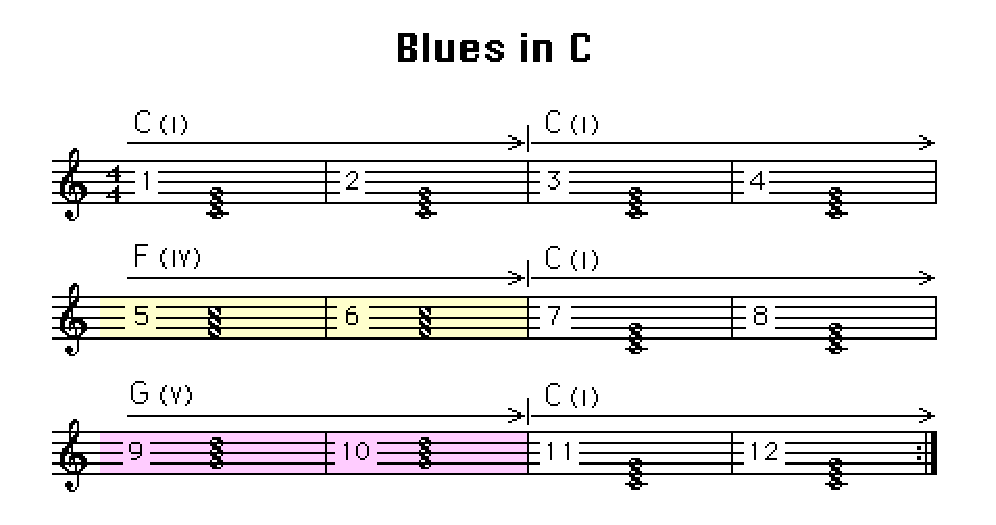
\includegraphics[height=85mm]{blues-example.pdf}
\captionfonts
\caption[Twelve Bar Blues Example]{Twelve Bar Blues Example}
\label{fig:blues-example}
\end{figure}

A human performer can often play with other performers just by listening to the music and discovering the chord progression, time signature and key signature innately. Computer performers have many ways of discovering key signature, chord progression, and time signature. The way that music is described in this system is through a time-signature, key-signature, tempo and chord progression. With these data the performer can make a prediction about what chord will be next and perform some music.

\section{Haskore}
\label{rw:haskore}

Haskore is a library written for Haskell used to describe, transcribe, and manipulate music~\cite{Haskore}. It uses a simple syntax to describe music and music related events. Haskore provides access to other library functions, in addition to providing a syntax for representing music. Some examples are a `transpose' function which moves the music up or down in pitch, and a `scale' function which makes the music longer or slower by a certain scale. These functions and other characteristics of the Haskore library were neglected in the work done here. Specifically, phrases, players, instruments, and the library functions were excluded from this work. 

Haskore's syntax is not exactly like the syntax used in the figure below ~\ref{fig:haskore-example}. The syntax has been changed to be akin to a list structure. In figure ~\ref{fig:haskore-example}, the first piece of music is a C Major scale where every note is performed for a duration of a quarter note. The second piece of music represents a C major chord followed by a G major chord with a half note length rest. When music is played 'in parallel', meaning it is chorded or there is some amount of time where the two notes are sounding simultaneously, the :=: symbol is used. Other music, like the scale example, is played 'in sequence' and the :+: symbol is used. The notes have a number value associated directly with the pitch, 2's and 3's in the example. This just describes which octave the pitch should be played in. The other number is the duration of the note. The :+: and :=: symbols can be used together, as seen in the chord example, to describe any kind of music. It should be noted that at the time of writing this the work in Haskore seems to be continuing with work in Euterpea here http://code.haskell.org/Euterpea/

\begin{figure}
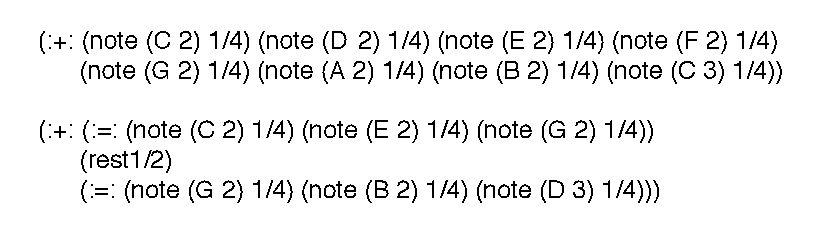
\includegraphics[height=45mm]{haskore-example.pdf}
\captionfonts
\caption[Haskore Example]{Haskore Example}
\label{fig:haskore-example}
\end{figure}

\section{Music}
\label{rw:music}
The most directly related work is \em{Band-out-of-a-Box}\em.~\cite{bob} This was a system that traded solos between a human musician and the computer performer. The goal was to create a learning model that could be trained on existing jazz musicians' improvisations. User performed improvisations are represented by variable-length trees. These trees record every note in every measure and then in the context of the measure describe a \em{Pitch Class,}\em an \em{Intervallic Motion,}\em and a \em{Melodic Direction.}\em The \em{Pitch Class}\em is just a tally of which notes were played and how many times the notes occurred. \em{Intervallic Motion}\em records the intervals, or distances between the pitches in each measure.  \em{Melodic Direction}\em has a rather complex way of recording descent and ascent of the pitches.  The \em{Melodic Direction}\em records the number of times successive pitches descend remain the same or ascend, three note sequences descend, remain around the same note or ascend, and finally the same for four note sequences. 

The work on \em{Band-out-of-a-Box}\em also included an experiment of using the learning framework with the variable-length trees and the three characteristics noted above. The interesting conclusion drawn from the experiment is that these three characteristics, \em{Pitch Class, Intervallic Motion,\em and  \em{Melodic Direction}\em are actually surprisingly useful at describing the activity and motion of a performers improvisation. Additional processing can be done over the data to discover what scales are used in what measures, how frequently those scales are used with certain rhythms and syncopations, etc. By learning all of these things the \em{Band-out-of-a-Box}\em was able to create a very complex improviser.

There has also been a fair amount of work done in recognizing melodies and repeating motifs~\cite{MelodicRecognition}. This work classifies a list of string matching problems and shows how they relate to multiple domains, but specifically music. Most relevant to this work is the problem listed as "Overlapping Repetition Identification." The problem consists of locating repetitions in the musical score or string. The solutions that are referenced account for repetitions in different voices, which compute in non linear time, and a more efficient solution of using 'tiles' to discover repeating segments. Similarly, there has been work done with a "sliding window" to lead to pattern discovery and matching~\cite{slidingWindow}. The solution here is to have a sliding window of cut pieces. A `join' function is also described which can concatenate patterns that are overlapping due to the cutting process. There has also been work done with music and databases~\cite{musicDB}. The work here describes a method of finding every repeating pattern in a piece of music. The results show that every repeating pattern in a piece of music with 1000 notes can be found in 10 seconds~\cite{musicDB}.

There is a very good overview of what current problems are in computer music and how they have been addressed here~\cite{Gerhard}. Of particular interest in section 8 where musical grammars are discussed. The conclusion is that more work needs to be done in key signature and time signature recognition as they are not simple problems. This work gets around those problems by using MIDI.

\section{Functional Reactive Programming}
\label{rw:frp}

Functional Reactive Programming, or FRP, is a programming paradigm that incorporates reactive elements in a functional language. [todo describe what a functional language is, reactive language] The languages used for this system are FrTime (pronounced 'Father Time')[citation] and Racket. 

FrTime is a functional reactive language written in Racket. [talk about FRan or whatever that graphics thing was.. grab some good frp research]

A lot of work has been done in formalizing reactive programming to ensure timely results~\cite{EventDriven}\cite{RealTime}. These works were driven by a desire to use a functional reactive language in robotics applications. The results of this work was a formalized method to ensure realtime results. The work described in this paper does not expand upon these works, but relies heavily on its basis and promises. The performer must react in realtime to events that are triggered just like a robot must react to external stimulus in realtime or else it will fall off a cliff. Luckily, preventing a robot from falling off a cliff is a lot like preventing a musician from playing a bad melodic phrase. This framework would not exist without this work.

\chapter{Implementation}
\label{Implementation}
The main advantages in using a reactive language for the implementation come at the highest level of the implementation. The system uses what essentially reduce to a small set of modules, the parser and the analyser, which are written in Racket, anytime a new event is triggered. 

The system requires a MIDI instrument connected to the users computer. On Mac OS X the CoreMIDI library is used to retrieve the MIDI data that the instrument outputs. On Linux, the user must also install Jackd (jackaudio.org) and manually connect the MIDI Instruments out port, through USB or some other interface, to DrRackets in port. At this point the MIDI data is parsed and concatenated to any MIDI data that has already been seen by the system. The parser outputs a correctly formatted piece of Haskore which is built up as the messages are received. 

The choice to use MIDI was made to avert the complex and unfinished work regarding pitch and time signature. MIDI provides the exact note number, so there is no need write signal processing software. The rhythm on the other hand provides slight problems because of the exactness with which MIDI data can describe time. MIDI provides 'on' and 'off' signals for each note. So by depressing middle C on a MIDI keyboard, the MIDI 'on' message is sent. When the key is released then the MIDI off message is sent. The duration between the 'on' and 'off' message is the duration of the note. For a performer playing in the time signature 4/4 with a tempo of 60bpm a quarter note should last for one second. Humans playing with these restrictions will most likely perform notes of different durations, but durations that approximate one second. Since MIDI is so exact it is possible to think that two quarter notes played in succession are actually two notes with a rest in between. To account for this human flexibility a method called quantization is used. Quantization in this system basically allows a range of values to be described as one specific value. So a quarter note in 4/4 at 60bpm can last anywhere from .9 to 1.1 seconds and still be a quarter note. 

At this point musical analysis takes place on the Haskore data to create a musical piece: a structure that holds possible key signature, a list of chords (the progression) and a time signature. As the user performs more of the piece the list of chords grows and the list of possible keys shrinks. The list of chords will grow indefinitely in the current implementation, but due to the repeating nature of music there is potential to use another piece of data in the piece to describe the form, apart from the chord changes. The key signature is strictly defined as having only notes that are harmonic to all the major and minor keys. That is, if a song in C major is being performed and an F\# is played as a chromatic passing tone C major would be excluded incorrectly from the list of possible key signatures. 

Some color notes will remove a key signature from the list of possible key signatures while others won't. Since some color tones are frequently used they are considered part of the key signature.  Specifically, in a major key the minor third and minor seventh are allowed to occur and the major key signature will still be considered diatonic. These two tones are allowed because of their frequent inclusion in jazz music. In a minor key the major sixth and major seventh are allowed to occur. These tones are allowed due to their inclusion in the melodic minor and harmonic minor scale. 

Musical form can be used by humans to predict the next chord that will be played. A human performer hears that other performers are playing the chords C d F G in succession and assumes that the song cycles through these chords the whole time. A human is able to do this because of pattern recognition. Computers are particularly good at matching patterns, but the patterns being matched have to be provided.

With the musical piece in hand, the system tries to create a musical fragment for performance. When the performance class is given a musical piece, it tries to predict, from the chord list that it has, what chords will be played by the user next. If it is able to predict some future chords then it writes a musical fragment that would adhere to the upcoming chord progression and performs it. So if a C major chord followed by a G major chord had previously been performed, then the next time the performer reads that a C major chord has just been played it will write music assuming that a G major chord is next. 

This presents our first problem with our solution. Every time that the system receives an event or a note, the entire piece of music, or every note that has been performed so far has to be parsed over to look for patterns. Instead of worrying about capturing every pattern that exists in the piece of music the system keeps track of patterns that it has seen and whenever it sees a new pattern it makes a note of how many measures of music it has seen so that the next time it iterates through the music it knows to start looking past that specified measure. The framework then tries to match the current chord progression against it's list of discovered patterns to predict what chords will be played next.This is akin to the tiling method that was mentioned earlier. The other, non linear methods described are too slow to be useful in a realtime setting. The sliding tile is fast enough, but slows down significantly as the size of the piece increases. This is also true with the database method which used matrices and took 10 seconds to match every pattern for 1000 notes. Since realtime execution is the priority here the sliding window method was simplified to account for just the recently seen measures. Another simplification and optimization is used to enhance the second pass of the music. The first pass finds new chord progressions to be added to the list of saved progressions that have been seen to be musical patterns. The second pass looks at the last couple of measures in the music and tries to match a discovered pattern to one that has been saved. This too, can slow down the realtime performance if enough patterns are saved. To get around this problem, only the ten most recent patterns are saved. 


The whole system works together with FrTimes event handling infrastructure. A sychable Racket event is made and setup through Racket's C API . This Racket event depends on MIDI messages. Anytime a MIDI message is sent from the user's instrument this Racket event is synced. The synchronization of this event sends a FrTime event to a FrTime event receiver. A function that takes the current value of the synchronized FrTime event and then parses, analyses and tries to perform with the output is mapped to every event that the FrTime event receiver receives through the use of the `map-e' function.

A problem arises at this point in the implementation. Since the FrTime event receiver will trigger the execution of the performer with every MIDI message it receives the system will create too much music. If the performer correctly predicts the upcoming chord progression for the next three chords it will also predict the correct chord progression when there are only two upcoming chords to predict and also one. In this way the performer will perform the same measure of music as many as three times (the last measure to predict). The other case that is of our concern is when the performer incorrectly predicts the upcoming chord changes. In this case, the performer could be playing music that doesn't adhere to the musical structure and will be distracting for the user and any listeners. Both of these issues reduce to the same problem. The system has many values to choose from at any point in the future and it must decide which value will be the 'best' at or before that time.

\section{Signal Handler}
\label {signal-handler}
To accommodate the problem of many values to choose from at each distinct point in time a signal handling module was developed. The problem can most simply be described as having many values for each distinct point in time, but only needing one. 

This signal handler requires a clock, an evaluation function that takes any number of arguments, a signal reference, and finally a base value. The clock is used to know when the value should change. The signal reference is shared between this signal handling interface and anyone interested in the value that is produced. This interface also provides a function `add-to-signal' which allows the programmer to add values to the signal at discrete points in the future. These future time values correspond to future time values of the clock that was passed as a reference to the signal handler at instantiation. Finally, the signal is set to the base value whenever the clock ticks and no values have been added to the signal for that instant in time. This prevents the system from performing the same musical fragment repeatedly until a new one arrives. 

In a simple example the value function would be the mathematical function `max.' This function always returns the largest of the values that were passed to it. So if the user of the signal handler called `add-to-signal' with the value 10 at time 1, and the value 3 at time 1, and the value 2 at time 1, then when the clock ticked to 1 the value of the signal would be 10 and only 10 because that is what max would return. 

For our use, the discrete values which need to be passed into the `add-to-signal' function should be small musical fragments. The value function should then choose between any possible musical fragments in the list of added values to choose the most musically appealing value.  With this tool the signal will only ever have one musical value at each discrete point in time. That value will then be performed and heard as the output of the system. 

\chapter{Experiment}
\label {experiment}
To find the implementation that is most appealing to the user of this system probably requires multiple executions with different functions controlling the output of the musical signal and different logic in the performer itself. A small experiment was performed with the system in hopes of meeting the author's definition of a musically pleasing performer. 

\section{Performers}
\label {performers}

Two different performers are used with each of the music value functions described below. The first one creates music depending on the chord changes that it was provided explicitly. This first performer looks for cadential patterns and writes music specific for those patterns. If no cadence is found it just plays the root of each change it sees for a whole measure. It does this for each note in the list of upcoming changes. If a cadence is found then depending on if it is an authentic cadence, a half cadence, or a deceptive cadence, it makes random music of random durations using the chord changes it assumes are to be performed up until the cadence, then writes specific music for the cadence taking advantage of the cadence. For example, if it is a half cadence it ends the phrase either on the third or fifth of the last chord.

The second performer makes melodies starting from the root note of the first chord that is predicted. It relies more heavily on the key signature than the first performer discussed. It stays in key or keys that have been provided by the analysis. This means that some of the notes will probably be out of the actual key signature. The way it constructs melodies is to randomly ascend and descend the the notes that are harmonic to the possible scales. All notes are given a duration of one eighth note. It performs like this for the duration of the provided upcoming changes. So if it were given a list of three chords it would make three measures worth of music in this fashion, but not necessarily adhere to the chord changes that were provided.

\section{Musical Value Functions}
\label {musical-value-functions}
Three different value functions were written for the experiment. Each function was used with each performer. 

The first function simply returns the value most recently added to the signal assuming that the performer will write better music when it is predicting chords that are temporally closer to what has actually been performed by the user.  

The next functions were inspired by the work done with ~\em{Band-out-of-a-Box.}\em This work closely mirrors the use of intervals and melodic direction although not as completely as was done previously~\cite{bob}.

The second function looks for the most rhythmically similar passages. As musical fragments are performed the duration of each note is tallied, keeping track of which rhythmic values have been most common. So if the first musical fragment consists of two quarter notes then that is added to the state. The function chooses passages that have notes over those that don't so that even if the rhythm is more consistent in a passage of nothing but rests, the passage that has actual music to play will be chosen. The next metric for the function is a simple addition of the number of rhythm values that have been seen to the ones to be chosen. So with the previous example, we had two quarter notes. Imagine two passages are being compared in this function. One has a quarter note and the other doesn't. The passage with the quarter note will be chosen and the state of rhythms that have been seen will reflect the two previously viewed quarter notes, the new quarter note about to be played, and whatever other rhythms the passage about to be performed consists of.

This function uses rhythm instead of pitches or intervals, in the way that ~\em{Band-out-of-a-Box}\em studied. By trying to copy the rhythms it has 'heard' it tries to mimic the human performer. A complimentary function could be written that performs rhythms that the human performer is not performing (e.g. triplets if the human plays quarter notes etc.)

The third function uses some simple knowledge about melody to choose which musical passage should be returned. Most melodies have a sort of rise or a fall in pitch that takes place over a few measures, giving the melody a contour. This function picks passages that have notes over those that don't for the same reasons as the second function. Initially, the function chooses passages that descend with equal probability as it chooses those that ascend. Once a direction has been chosen though, it tries to continue that direction for three signal values. After those three signal values the probability to go up or down again is reset to zero so that the melody can rise and fall and does not simply careen off in one direction. This function chooses between different passages that head in the same direction by using a distance metric. Melodies often times jump from one note to a note twelve tones above or below it. Other times, melodies will meander around a central note with small hops and scalar motions. This function chooses between passages that have the correct direction by trying to keep the melodic distance travelled small. When looking for a passage that descends, a passage that descends a distance of ten will always win over a passage that ascends a distance of one. Deciding between two passages that descend, one a distance of ten, the other a distance of three, the less distant descent will be chosen. Distances are defined as the most extreme distance in the passage.

While ~\em{Band-out-of-a-Box}\em used all of the data to learn and train an improviser to act like the one in the piece, this function uses only the data it has 'heard' played by itself to choose the next passage to play. 

\section{Music Performed}
\label{music-performed}
For simplicity the music that was performed for the experiments was all the same and easy to replicate. The human experimenter performed in 4/4 at a tempo of 120 beats per minute. Two different phrases were performed to determine the different qualities from the different computer performers and music value functions. 

The first phrase that was performed was simply a repetition of C major and G major. After the computer had been performing for twenty seconds or so, the human performer began playing D major and A major chords at the same rate. After the computer had sufficiently adjusted to the new key signature and chords the human jumped back to C major and G major. 

The other phrase that was performed was more complicated. A simple cadential pattern was developed and cycled through. The chords C major, d minor, F major, and then G major were played and then were followed by the chords C major, F major, G major, and finally C major again. This is a simple pattern that includes both a half cadence and a perfect authentic cadence. Each chord was held for two beats or one second.

\chapter{Results}
\label{results}
This section describes how the music the different performers and music value functions were perceived first with the simple chord progression of C major to G major that included a change in key signature to D major, and then the more complicated cadential chord progression. The section is organized primarily by the music value functions. Within the discussion of each function each chord progression is discussed with each performer. 

The first chord progression was the simple repetition of C major and G major which then switched to D major and A major and finally returned to C major and G major. The first music value function, the function that returned the most recently created music was tested with both the cadential performer and the scalar performer.The cadential performer sounded best with this function and the third function with these chord changes. The phrases that it constructed were rhythmically complex, due to the randomness, and disjoint, including a fair amount of rest time.The scalar performer performed modestly playing meandering ascending and descending patterns. With the more complex musical phrase the music created was aesthetically unbearable. It had no direction and lacked melody. With both of the performers this more complex phrase did not produce any good results. With the more simple musical phrase this function was not as unbearable, but equally was not particularly interesting.

The second function, the function based on previous rhythmic values was able to give the cadential performer some much needed rhythmic structure. The melodies created were still abstract at best, having no real direction or personality but by restricting the rhythm just slightly like this function does the music created sounded less random and did not make large leaps in rhythmic duration as frequently as the previous experiment's phrases did. The scalar performer had no effect with this function as all of the notes are given a duration of an eighth note. This performer did not sound much different here than it did in the previous function. With the more complex musical phrase this function actually produced better results than the previous function. The structure that the function gives by choosing phrases based on rhythmic similarity helps to keep music intelligible. The first performer was a better use of the framework. The second performer sounded too chromatic and almost atonal due to the freedom of note choice. The second performer could be improved in this case by changing what is defined as notes that are in the key signature. If the key signatures were more limited then this, the second performer would have less keys to choose for this phrase. Since the key signature is loosely discovered over a longer period of time and includes so many color notes the possible key signatures during the performance are still to many and lead to particularly unpleasing chromatic passages.

The third function, the function which chooses phrases for their general melodic direction had the most interesting effect on the scalar performer. The cadential performer performed poorly with this function because phrases that jumped large intervals were played more frequently, a choice made by the function's desire to continue passages in a general direction. This jumping of large intervals was not pleasant or very creative. The scalar performer on the other hand, which creates randomly ascending and descending patterns was actually given some character with this function. Normally this performer just meanders in either direction. This function gave these meandering phrases some overall direction. The music would move up and down having a larger form meandering which was probably the most musical sounding of all of the different combinations. With the more complex phrase once again, the cadential performer produced better music. The passages that were created had better melodic direction and were less confusing than the first function with the cadential performer. The scalar performer was confused still due to the many possible key signatures. This cadential performer suffered from the same limitation as described in the second performer of having too many possible key signatures.  A slight improvement would be to add some slight randomness to the rhythm that is chosen for the duration of the notes so that the music does not sound so metronomic. 

The first function provided the most consistent results for the simple chord progression. Since this function always chooses the most recent piece of music the phrases are shorter, usually one measure. This function is probably not the best or worst choice for any particular performer that a user could create. The music that it chooses tends to be very consistent though most likely due to the performer's logic for the final chord in a progression being limited by the cadential performer and just the static nature of the music created by the scalar performer.  With the more complex chord progression this function performed poorly.

The second function is a fairly good choice as it provides structure to the music. This is also its greatest weakness though. The music that is chosen can sound annoying and too repetitive. Since it doesn't use the notes that are chosen, just the duration of the notes the melody can jump from one place to another. This did produce fairly consistent results with the more complex phrase of music though. The cadential performer in particular produced interesting music that was easier to listen to than the first function. Obviously this function has no real effect on the scalar performer as every note in the passages that are created have the same eighth note duration.

The third function does have an effect on the scalar performer. The music can become boring and annoying though with this performer because the movement tends to be centered around one or two notes. This could be improved by adding a jump or two which would add some much needed randomness and surprise to this performer. This function worked well with the cadential performer as well. This functions weakness seems to be centered around its concern for rhythm. The music choices can leave confusing pauses in the performance due to the randomness that the cadential performer uses in its duration choice. If the cadential performer were less random with its rhythm choice, or this function were more concerned with the note duration the results would probably be the best. Just as the last function did not care about pitch choice this one does not care about note duration. The combination of both of these functions is worth investigating. 

With the simple passage of music the best combinations were the scalar performer with the third function and the cadential performer with either the first or second function. When more complex music was used the scalar performer produced unpleasant music. The cadential performer was best with either the second or third function. The cadential performer could be included by using less randomness in its rhythm choice. If the rhythms that were used were more consistent than the performer would sound less confusing and disconnected. Alternatively, the scalar performer should be more rhythmically diverse. The second and third function could also be combined to make a new function. 

Probably the most useful addition to the music value functions would be some sort of "kill switch." Since the performer continued to play phrases in the incorrect key signature after the piece had modulated the music that it performed sounded particularly dissonant. This was particularly noticeable when the human performer switched from playing C major and G major to D major and A major. Since the patterns that had been predicted by the framework were long enough the performer played music based on C major and G major chords for close to five seconds before reacting and writing new music with the new D major A major pattern. The music value functions have no perception of what chord is currently being played and only choose music based on the metric of general musicality over all key signatures and chord changes. A secondary function could be included into each music value function that would run before the functions experimented with ran. This secondary function would take the list of possible music to perform and the chord changes that the music was created with and compare it to the current state of the analysed piece of music. If the upcoming changes were different from the chords that were currently being performed the music that was made with those changes would be excluded from the second pass, the music value functions that decide which to play based purely on musical quality. 

The patterns that are discovered may be to simplistically defined. Since some progressions do not change chords every measure the framework can consider not moving from a chord a pattern. This resulted in some notes being played syncopated whenever a chord was changed. With the more complex chord changes in particular the system would occasionally play just a note or two on the second beat, predicting that the chord would remain for longer than a measure. It predicted this because the chords lasted two measures each. The patterns that were discovered were small one chord patterns that reflected the chord not changing every measure.t

The pattern discovery and matching suffers due to the realtime restriction. Many larger patterns are neglected in favor of realtime execution. Once the system finds any pattern in the music in which it hasn't discovered a pattern yet it updates the marker of where to look next. So if a pattern that was previously found (e.g. C G) is then later found again, the marker, which keeps track of where to start looking for patterns next time, is updated to exclude the music containing the newly discovered pattern from future searches. This denies the system the opportunity to ever discover any larger form patterns. The irony here being that by saving one or two larger form patterns in a piece of music all of the smaller ones would be irrelevant as the larger form pattern would encompass all of the smaller ones excepting some cadential passages and variations. 

Only saving ten patterns also provides a disservice to the system at times. The advantage with only keeping track of the last ten patterns is that if a piece modulates to a different key, or if it changes progressions, the performer will be able to play along quite quickly because the newest patterns will be easily retrieved. The main problem is that all of the patterns that were relevant previously may be thrown out if the piece stays in the new key area for enough time. Often times pieces will move to a different key area, using new chord progressions and then move back to the original material. If all of the patterns were saved then when the piece moved back to the original material the performer would be able to play almost instantaneously. 

Some problems definitely arise due to the implementation of key signature discovery. F\# which is not included in the major key list for C major, can often arise as a chromatic passing tone, or as a part of a D major chord being used to tonicize G. Tonicization is when a chord other than the tonic or root, or name of the key signature is temporarily emphasized as if it were the key signature. A\# can also be a chromatic passing tone which would exclude the possibility of C major. G\# should be included in the C major list as well. G\# is used in a C major chord sometimes to move from a C major chord to an a minor chord. The only note now not belonging to C major would be C\# but this note also should be included because of Neapolitan 6th chords, used as a subdominant substitute.

If we were to include all of these possibilities then every key signature would have every note as a possibility meaning we would never know what key signature the piece is in. A secondary tool should probably be developed to allow for a few instances of these less commonly used color tones but not allow for so many that C major and F\# major are both being considered as possible key signatures after four or five bars of music. A signal could be used that would allow for notes outside of the strict key signature to be played. The signal would work somewhat like a semaphore, having a value that gets decremented by the performance of a color tone, and incremented (up to a point) by a delayed computation. 

The chordal analysis could be upgraded to include chords that don't function with just one pass over the piece, reading from left to right. Some chords, namely secondary dominants and the Neapolitan sixth function differently depending on where the music goes after the chord sounds. D\# major, a secondary dominant in the key of C major, could function as a chord used to tonicize G major, or as a chord in a modulation (changing of key signature) to G major. 

The simple solution that was used to handle all of these issues was to neglect any of the logic needed to correctly interpret and analyse the music and instead only remember the last ten patterns that have been seen. In this way, if a piece modulates the performer is 'confused' for a moment and then with the new patterns it has accumulated, begins playing anew, in the new key signature. 

\chapter{Future Work}
\label{future}

The future work will take two directions. Firstly, the analysis of the music being performed by the human performer can be improved with some better logic from previous work done in melodic improvisation and recognition~\cite{MelodicImprovisation}~\cite{MelodicRecognition}. By recognizing melodies that the human performer plays, and relating them to specific chord changes, the performer could harmonize with the human performer by predicting that the melody will return the next time that the chord progression comes around. This would also allow for some improved improvisation by manipulating melodies with transposition, retrograde, inversion and combinations of these manipulations. The static implementation of what is or is not harmonic to a key signature should be loosened up to provide chromatic notes and more color tones. This would require some overhauling of how key signature is discovered. 

With the pattern matching issues, a modified join function could be used to help put smaller patterns together and make larger ones~\cite{slidingWindow}. This work would have to be modified, but an asynchronous joining behavior could run trying to put smaller patterns together to make larger ones which could then be permanently saved. This would solve more than one problem described in the results. Firstly, by adding these larger form fragments the confusion of when thematic or original material returned after a period of time where the piece was developing new material would be remedied. The performer would know to look for larger forms if no small patterns matched. The behavior could also be triggered anytime the pattern list reached its full size. 

The music value functions could be improved with more complex models. For example, the rhythmically minded performer could pick passages that leave a distribution that approximates a normal curve. 

Secondly, the system itself can be improved to take advantage of other technologies that already exist. Multiple human performers accompanied by the system. Multiple computer performers each playing with a different voice (saxophone, clarinet, etc.) The biggest roadblock to this work is finding an interface that can handle all of the MIDI traffic. Rewriting the system to have more than one performer would not require much more work, a controller module could handle this. 

The most pressing issue, and probably the most interesting is to make this framework so easy to use that non programmers could program performers. This can be accomplished by using a very small, domain specific language that musicians would understand given that they know some music theory. The musical value functions require a higher level language, but with a few preprogrammed into this system already users could simply select different functions and decide which is best for the performer that they are writing. 

In writing the performers the user could be provided with a small library of useful functions for creating notes. In the scalar performer created here, two functions `get-next-note-in-scales' and `get-prev-note-in-scales' were created which given a list of possible key signatures and a note return the next, higher frequency, pitch in any of the provided scales or previous, lower frequency pitch in any of the scales. Other very simple functions could be written to create a library for the creation of performers. 

The signal handler could also be used in many other domain specific applications like robotics and facial recognition. 

\chapter{Conclusion}
\label{conclusion}


% ------------- End main chapters ----------------------

\clearpage
\bibliography{bibliography}
\bibliographystyle{plain}
%\addcontentsline{toc}{chapter}{Bibliography}

\end{document}